\chapter{Trees and Distance}

\section{Basics}%
\label{sec:2.1}

We will begin with some terminology.
A graph without any cycle is said to be \textbf{acyclic}. A \textbf{forest} is an acylic graph. A \textbf{tree} is a connected acyclic graph. A \textbf{leaf} is a vertex of degree 1. A \textbf{spanning subgraph} is a subgraph containing all vertices.

\begin{theorem}
	For a graph of order $n$, the following are equivalent and characterize trees with $n$ vertices:
	\begin{enumerate}
		\item $G$ is connected and has no cycle
		\item $G$ is connected and has $n-1$ edges.
		\item $G$ has $n-1$ edges and no cycles
		\item $\forall u,v \in V(G)$, $G$ has exactly one $(u,v)$-path
	\end{enumerate}
\end{theorem}
Though the proof will be omitted, we obtain some interesting properties from this theorem:
\begin{enumerate}
	\item Every edge in a tree is a cut-edge.
	\item Adding one edge to a tree forms exactly one cycle.
	\item Every connected graph contains a spanning tree.
\end{enumerate}

\begin{proposition}
	If $T$ is a tree with $k$ edges and $G$ is a simple graph with \(\delta(G) \ge k\), then $T$ is a subgraph of $G$.
\end{proposition}

\begin{proof}
	We prove by induction on $k$.\\
	\noindent
	\textbf{Base Case $k = 0$}: $T$ is just one vertex. Thus $G$ must contain $T$.\\
	\noindent
	\textbf{Induction Step}: Assume true for all values smaller than $k$. Let $u$ be a leaf of $T$ and let $uv \in E(T)$ and $T' = T - u$. By the induction hypothesis $G$ contains a subgraph $H \cong T'$. As $d(v) \ge k$, $v$ must have a neighbour $x$, in $G$ but not in $V(T')$ as $|V(T')| = k$. Add the edge $vx$ to the subgraph $H'$. This shows that $H \cong T$ is a subgraph of $G$.
\end{proof}

The \textbf{distance} between two vertices $u$ and $v$ is the length of the shortest path from $u$ to $v$ in $G$. We denote the distance $d_{G}(u,v)$ or $d(u,v)$. We define the distance function to give value $\infty$ if there exist no $(u,v)$-path. We say the \textbf{eccentricity} of a vertex $u$ is $\epsilon(u) = \max_{v \in V(G)}\{d(u,v)\}$. I.e., given a vertex $u \in V(G)$, the eccentricity of $u$ is the maximum length from $u$ to all other vertices in $G$. The \textbf{radius}, denoted $rad(G)$ is the minimum eccentricity for all vertices in $G$, i.e., $\min_{u \in V(G)} \{\epsilon(u)\}$. On the other hand is the \textbf{diameter}, which is the \textit{maximum} eccentricity.

\begin{theorem}
	Let $G$ be a simple graph. If $diam(G)\ge 3$, then $diam(\overline{G}) \le 3$.
\end{theorem}

\begin{proof}
	Assume $G$ is simple and $diam(G) \ge 3$. Thus there must exist $u,v \in V(G) \mid d(u,v) \ge 3$. This means that there is no third vertex which is adjacent to both $u$ and $v$, as this would give a distance of length 2. So, in $\overline{G}$, every vertex is adjacent to either $u$ or $v$ and $uv \in E(\overline{G})$. Hence, in $\overline{G}$ it must be that $diam(G) \le 3$.
\end{proof}

The \textbf{center} of a graph $G$ is the subgraph induced by the vertices of minimum eccentricity. Thus, it is a subgraph containing the vertices whose maximum distance to all other vertices is the shortest of all vertices.

\begin{theorem}
	The center of a tree is a vertex or an edge (rather than a set).
\end{theorem}

The \textbf{Wiener index} is another known parameter of a graph, specifying the sum of distance between all pairs of vertices: $W(G) = D(G) = \sum_{u, v\in V(G)} d_{G}(u,v)$.

\begin{theorem}
	Among trees with $n$ vertices the Wiener index is minimized by stars and maxmized by paths.
\end{theorem}

\section{Spanning Trees and Enumeration}%
\label{sec:label}

We will now turn to the question of how many spanning trees there are with $n$ vertices. Recall that given $n$ vertices, there are $2^{\binom{n}{2}}$ graphs. When $n = 3$, there are three spanning trees. With $n = 4$ there are $16$. We will now present \textit{Cayley's Formula}.

\begin{theorem}[Cayley's Formula (1889)]
	For a set $S \in \mathbb{N}$ of size $n$, there are $n^{n-2}$ trees with vertex set $S$.
\end{theorem}
We will prove this using Prüfer codes. This proof is not Cayley's, but instead Prüfers from 1918.

For an example, given $n = 5$, there are $5^{5-2} = 5^{3} = 125$ distinct spanning trees.

We start by defining Prüfer codes. We obtain the Prüfer code by removing the leaf of the smallest index (each vertex is given a unique index), and record the unique neighbour.


\begin{figure}[ht]
	\centering
	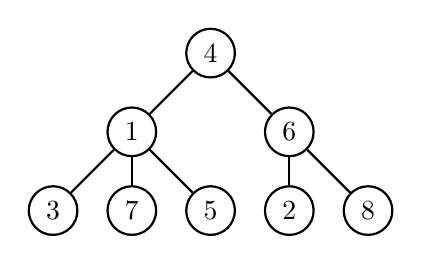
\begin{tikzpicture}[node distance={30mm}, thick, main/.style = {draw, circle}]

		\node[main] (4) at (0,0) {4};
		\node[main] (1) at (-1,-1) {1};
		\node[main] (6) at (1,-1) {6};
		\node[main] (3) at (-2,-2) {3};
		\node[main] (7) at (-1,-2) {7};
		\node[main] (5) at (0,-2) {5};
		\node[main] (2) at (1,-2) {2};
		\node[main] (8) at (2,-2) {8};

		\draw (4) -- (1);
		\draw (4) -- (6);
		\draw (1) -- (3);
		\draw (1) -- (7);
		\draw (1) -- (5);
		\draw (6) -- (2);
		\draw (6) -- (8);
	\end{tikzpicture}
	\caption{\label{fig:pruferexample} A tree with Prüfer code \texttt{6 1 1 1 4 6}}.
\end{figure}

In Figure~\ref{fig:pruferexample} we obtained the Prüfer code \texttt{6 1 1 1 4 6} by following the algorithm described earlier as such:
\begin{enumerate}
	\item Remove 2 (the smallest leaf), record \texttt{6}
	\item Remove 3, record \texttt{1}
	\item Remove 5, record \texttt{1}
	\item Remove 7, record \texttt{1}
	\item Remove 1 (as it is now a leaf), record \texttt{4}
	\item Remove 4 (as it is now a leaf), record \texttt{6}
	\item We are now left with only two vertices and an edge between them, terminating the algorithm.
\end{enumerate}

From this it is clear that every spanning tree gives a unique Prüfer code. We will also show that every $(n-2)$-tuplewith entries from $[1 \ldots n ]$ gives a unique spanning tree, with that code as it's Prüfer code. This would imply that the number of trees is the same as the number of codes, which is $n^{n-2}$. Our next task is to show how to create a spanning tree with a given Prüfer code. Given the Prüfer code from Figure~\ref{fig:pruferexample} we have \texttt{6 1 1 1 4 6}. Given a vertex $i$, the degree of this vertex is the number of occurences it has in the Prüfer code $+1$. This can be shown by induction on $n$, where the base case is $n=2$. Thus, given the indicies of the vertices we can reconstruct the spanning tree as follows:

Assume we are given the Prüfer code \texttt{6 1 1 1 4 6}. We can find the leaves quickly, as they are $[1 \ldots n] \setminus \{1, 4, 6\} = \{2, 3, 5, 7, 8\}$. This must mean that $2$ was the first vertex to be deleted, and thus the first edge deleted was $26$. Thus we can add the edge $26$. We can now remove the first 6 from the code. The remaining code is \texttt{1 1 1 4 6}. We know the next leaf is 3, and thus it must have an edge to 1. We add the edge $13$ and remove the first 1 from the list, given us \texttt{1 1 4 6}. If we continue this process, we get back to the original tree.

While this has not been a formal proof (such can be found in the book), this should give the correct intuition.

\begin{corollary}
	Given positive integers $d_{1}, d_{2}, \ldots, d_{n}$ summing up to $2n-2$, there are exactly $\frac{(n-2)!}{\Pi (d_{i}-1)!}$ trees with vertex set $[1 \ldots n]$ such that vertex $i$  has degree $d_{i}$ for each $i$.
\end{corollary}

How many spanning trees exist with degrees \texttt{1 3 1 2 1}? If $T$ is a tree with degrees \texttt{1 3 1 2 1}, then $|E(T)| = \frac{\sum d_{i}}{2} = 4$ (from Degree-Sum Formula) so $|V(T)| = |E(T)| + 1 = 5$.

\begin{equation*}
	\frac{(n-2)!}{\Pi (d_{i}-1)!} = \frac{(5-2)!}{(1-1)!(3-1)!(1-1)!(2-1)!(1-1)!} = \frac{6}{2} = 3
\end{equation*}

What about if we want to know about the number of spanning trees in a general graph, rather than just in complete graphs?

\begin{definition}[Contraction]
	Let $G$ be a graph and let $e = uv$ be an edge in $G$. A \textbf{contraction} of $e$ replaces $u$ and $v$ with a single vertex whose incident edges are the edges other than $e$ that are incident with either $u$ or $v$.
\end{definition}

The graph resulting from a contraction is written $G \cdot e$ (assuming $e$ is the edge contracted). The resulting graph has one edge and one vertex less than $G$.

Let $\tau(G)$ be the number of spanning trees in $G$.

\begin{proposition}
	Let $G$ be a graph and let $e \in E(G)$ be a non-loop. Then \(\tau(G) = \tau(G -e) + \tau(G \cdot e)\)
\end{proposition}

\begin{proof}
	\(\tau(G-e)\) counts the number of spanning trees not using $e$. \(\tau(G \cdot e)\) counts the number of spanning trees using $e$.

	This holds as:
	\begin{enumerate}
		\item $\tau(G-e)$ counts spanning trees without using $e$:
		      \begin{itemize}
			      \item Removing the edge $e$ eliminates the possibility of any spanning tree using $e$. So \(\tau(G-e)\) directly counts the number of spanning trees that don't rely on this edge.
		      \end{itemize}
		\item \(\tau(G \cdot e)\) counts spanning trees using $e$:
		      \begin{itemize}
			      \item If a spanning tree in $G$ uses $e$, the contracting $e$ simplifies the graph by merging its endpoints. The resulting spanning tree is a smaller tree on the contracted graph. By reversing the contraction (i.e., adding back the edge) the spanning tree corresponds to a spanning tree in $G$ that uses $e$.
		      \end{itemize}
	\end{enumerate}
\end{proof}

\begin{theorem}[Matrix Tree Theorem]
	Let $G$ be a loopless graph with vertex set $v_{1}, v_{2}, \ldots, v_{n}$. Let $a_{i,j}$ be the number of edges between $i$ and $j$, $i \ne j$. Let $Q$ be the matrix with entries $-a_{i,j}$ when $i \ne j$, and $d(v_{i})$ when $i = j$. Let $Q^{*}$ be the matrix obtained from $Q$ by deleting row $s$ and column $t$. Then \(\tau(G) = (-1)^{s+t} det(Q^{*})\).
\end{theorem}
We omit the proof.

\begin{conjecture}[Ringel, 1964]
	If $T$ is a fixed tree with $m$ edges, then $K_{2m+1}$ decomposes into $2m+1$ copies of $T$.
\end{conjecture}

This conjecture is still open, and there has not been found a solution yet.

\begin{definition}[Graceful Labeling]
	A \textbf{graceful labeling} of a graph $G$ with $m$ edges is a function $f : V(G) \rightarrow \{0,1, \ldots, m\}$ such that distinct vertices receive distinct numbers and $\{|f(u) - f(v)| : uv \in E(G)\} = \{1,2, \ldots, m\}$
\end{definition}

A graph is said to be \textbf{graceful} if it has graceful labeling.

\begin{conjecture}[Graceful Tree Conjecture]
	Every tree has a graceful labeling.
\end{conjecture}


\begin{figure}[ht]
	\centering
	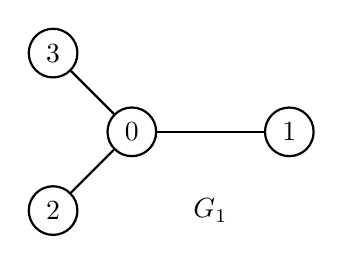
\begin{tikzpicture}[node distance={30mm}, thick, main/.style = {draw, circle}]

		\node[main] (3) at (-1,1) {3};
		\node[main] (2) at (-1,-1) {2};
		\node[main] (0) at (0,0) {0};
		\node[main] (1) at (2,0) {1};
		\node[] (g) at (1, -1) {$G_{1}$};

		\draw (3) -- (0);
		\draw (2) -- (0);
		\draw (1) -- (0);
	\end{tikzpicture}
	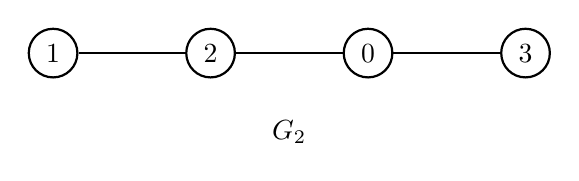
\begin{tikzpicture}[node distance={30mm}, thick, main/.style = {draw, circle}]

		\node[main] (3) at (-4,0) {1};
		\node[main] (2) at (-2,0) {2};
		\node[main] (0) at (0,0) {0};
		\node[main] (1) at (2,0) {3};
		\node[] (g) at (-1, -1) {$G_{2}$};

		\draw (3) -- (2);
		\draw (2) -- (0);
		\draw (1) -- (0);
	\end{tikzpicture}
	\caption{\label{fig:gracefullabelingexample} Two Graphs, $G_{1}$ and $G_2$, both with graceful labeling.}.
\end{figure}

In Figure~\ref{fig:gracefullabelingexample} you can see two graphs, both with graceful labeling.

\begin{theorem}
	If a tree $T$, with $m$ edges has a graceful labeling, then $K_{2m+1}$ can be decomposed into $2m+1$ copies of $T$.
\end{theorem}

We omit the proof.

Graceful labelings are known for all stars and paths, as well as all \textbf{caterpillars}. A caterpillar is a tree which contains a path (called the spine) which is incident with all edges. Note that both stars and paths are caterpillars.

\section{Optimization}%
\label{sec:2.3}

This section is about algorithms, whose proofs should already be known by now (and therefore are not part of the syllabus). There will therefore not be any proofs, only the algorithms themselves.

We start with \textit{Kruskal's Algorithm}, (Algorithm~\ref{alg:Kruskal}) which finds a minimum spanning tree on edge-weighted graphs.

\begin{algorithm}
	\caption{\label{alg:Kruskal}Kruskal's Algorithm for Minimum Spanning Trees}
	\begin{algorithmic}[1]
		\STATE \textbf{Input:} A weighted connected graph.
		\STATE \textbf{Idea:} Maintain an acyclic spanning subgraph $H$, enlarging it by edges with low weight to form a spanning tree.
		\STATE Consider edges in nondecreasing order of weight, breaking ties arbitrarily.

		\STATE \textbf{Initialization:} Set $E(H) = \emptyset$.
		\WHILE{$H$ is not connected}
		\STATE Select the next cheapest edge.
		\IF{the edge joins two components of $H$}
		\STATE Include the edge in $H$.
		\ELSE
		\STATE Discard the edge.
		\ENDIF
		\ENDWHILE
		\STATE Terminate when $H$ is connected.
	\end{algorithmic}
\end{algorithm}

We next look at \textit{shortest path} algorithms. We begin by looking at \textbf{Dijkstra's Algorithm}, (Algorithm~\ref{alg:dijkstra}) which finds the shortest path from any given vertex to all other vertices.


\begin{algorithm}
	\caption{\label{alg:dijkstra}Dijkstra's Algorithm for Shortest Paths from a Single Vertex}
	\begin{algorithmic}[1]
		\STATE \textbf{Input:} A graph (or digraph) with nonnegative edge weights and a starting vertex $u$. The weight of edge $xy$ is $w(xy)$; let $w(xy) = \infty$ if $xy$ is not an edge.
		\STATE \textbf{Idea:} Maintain the set $S$ of vertices to which a shortest path from $u$ is known, enlarging $S$ to include all vertices. Maintain a tentative distance $t(z)$ from $u$ to each $z \notin S$, being the length of the shortest $u$-$z$ path yet found.

		\STATE \textbf{Initialization:} Set $S = \{u\}$, $t(u) = 0$, and $t(z) = w(uz)$ for all $z \neq u$.
		\WHILE{$S \neq V(G)$ \textbf{and} $t(z) \neq \infty$ for all $z \notin S$}
		\STATE Select a vertex $v$ outside $S$ such that $t(v) = \min_{z \notin S} t(z)$.
		\STATE Add $v$ to $S$.
		\FOR{each edge $vz$ with $z \notin S$}
		\STATE Update $t(z)$ to $\min\{t(z), t(v) + w(vz)\}$.
		\ENDFOR
		\ENDWHILE
		\STATE At the end, set $d(u, v) = t(v)$ for all $v$.
	\end{algorithmic}
\end{algorithm}

Next we look at breadth-first search (Algorithm~\ref{alg:bfs}), which produces a result much like Dijkstra's algorithm, except it only works on graphs without edge-weight (or edge-weight = 1).

\begin{algorithm}
	\caption{\label{alg:bfs}Breadth-First Search (BFS)}
	\begin{algorithmic}[1]
		\STATE \textbf{Input:} An unweighted graph (or digraph) and a start vertex $u$.
		\STATE \textbf{Idea:} Maintain a set $R$ of vertices that have been reached but not searched, and a set $S$ of vertices that have been searched. The set $R$ is maintained as a First-In First-Out list (queue), so the first vertices found are the first vertices explored.

		\STATE \textbf{Initialization:} Set $R = \{u\}$, $S = \emptyset$, and $d(u, u) = 0$.
		\WHILE{$R \neq \emptyset$}
		\STATE Search from the first vertex $v$ of $R$.
		\FOR{each neighbor of $v$ not in $S \cup R$}
		\STATE Add the neighbor to the back of $R$.
		\STATE Assign $d(u, v) + 1$ to the distance of the neighbor.
		\ENDFOR
		\STATE Remove $v$ from the front of $R$ and place it in $S$.
		\ENDWHILE
	\end{algorithmic}
\end{algorithm}

The \textbf{Chinese Postman Problem} is a problem named in honor of Chinese mathematician Guan Meigu, who first posed the problem in 1962. The problem is the following: Given a graph $G$, find a \textit{closed walk} that uses each edge \textit{at least once} of \textit{minimum total weight}.

%%% Local Variables:
%%% mode: latex
%%% TeX-engine: luatex
%%% TeX-command-extra-options: "-shell-escape"
%%% TeX-master: "main"
%%% End:
